\documentclass{article}
\usepackage[utf8]{inputenc}
\usepackage{graphicx}

\begin{document}
\section*{Punto 2}
En este problema, se nos dice que la venta de armas a naciones hostiles por parte de estadounidenses es un crimen. Además, se nos da la información de que Corea del Sur es una nación hostil y que el Coronel West, que es estadounidense, les vendió todos sus misiles. A partir de esta información, podemos usar Prolog para determinar si el Coronel West es un criminal.

Primero, necesitamos definir algunos hechos en Prolog. Sabemos que Corea del Sur es una nación hostil y que los misiles son un tipo de arma, así que podemos representar estos hechos como:

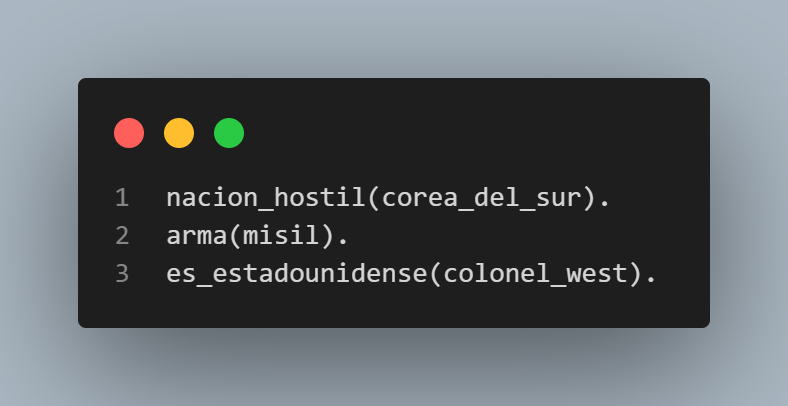
\includegraphics[width=0.5\linewidth]{./img/code.png}

Luego, necesitamos definir una regla que determine si alguien vende un arma a una nación hostil. En este caso, solo es un crimen si la persona que vende es estadounidense. Podemos representar esto como:

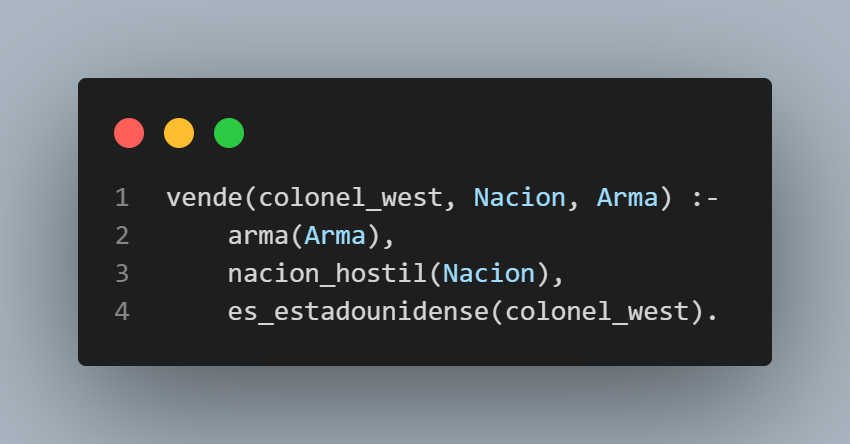
\includegraphics[width=0.5\linewidth]{./img/code1.png}

En esta regla, vende es el predicado que indica que alguien vende un arma a una nación, colonel\_west es el nombre del vendedor, Nacion es el nombre de la nación compradora, y Arma es el tipo de arma que se vendió. La regla establece que alguien vende un arma a una nación si la nación es hostil, el tipo de arma se corresponde con el objeto "misil" que hemos definido y si la persona que vende es el Coronel West y es estadounidense.

Finalmente, podemos definir una regla que determine si alguien es un criminal. Esta regla simplemente verifica si la persona vende un arma a una nación hostil y es estadounidense. Podemos representar esto como:

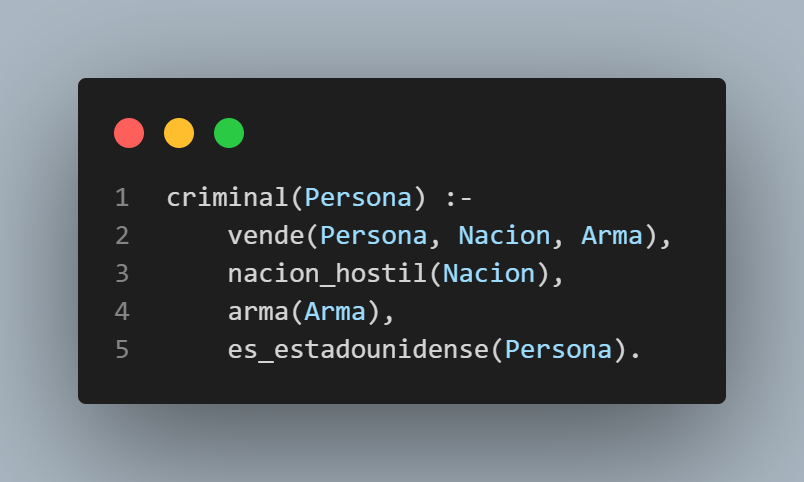
\includegraphics[width=0.5\linewidth]{./img/code2.png}

En esta regla, criminal es el predicado que indica si alguien es un criminal, y Persona es el nombre de la persona que estamos evaluando. La regla establece que alguien es un criminal si vende un arma a una nación hostil, el tipo de arma es el objeto "misil" que hemos definido, es estadounidense y se cumple la regla vende.

Finalmente, podemos hacer una consulta para verificar si el Coronel West es un criminal. Podemos representar esto como:

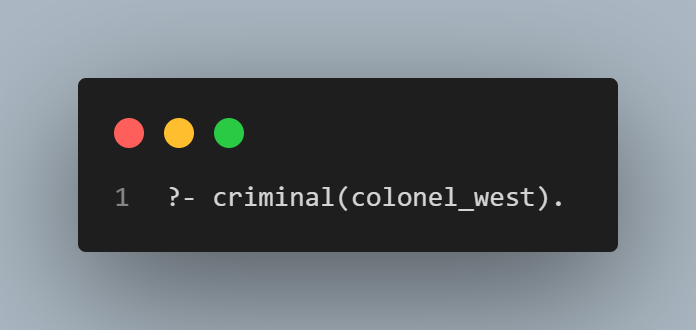
\includegraphics[width=0.5\linewidth]{./img/code3.png}

Esta consulta preguntará si el Coronel West es un criminal según la regla que hemos definido. Si se cumple la regla, Prolog nos responderá con "true", lo que significa que el Coronel West es un criminal. Si no se cumple la regla, Prolog nos responderá con "false", lo que significa que el Coronel West no es un criminal.
\end{document}